\documentclass[a4paper,12pt]{article}


\usepackage{dcolumn}
\usepackage{pdflscape}
\usepackage{graphicx}
\usepackage{hyperref}
\hypersetup{colorlinks=TRUE,
linkcolor=blue,
urlcolor=blue,
citecolor=blue,
}
%\usepackage{geometry}

\begin{document}

\title{To be decided}

\maketitle


\begin{abstract}
A relevant question in the study federal politics is whether
sub-national outcomes influence national outcomes. One important
channel of influence is the possibility of a coattail effect in the
electoral dimension. In this paper we analyze the specific case of
Argentine election. We  focus on the type of reverse coattail
effect that runs from gubernatorial (state-wide) election
to presidential (nation-wide) elections.
\end{abstract}


% \section{Comentarios Marcelo}

% \begin{itemize}
% \item Cómo se explica el signo negativo de “core” en Table 1?
% \item Problema de variable omitida (causalidad espúrea): identificación partidaria (tanto el presidente como el gobernador pueden recibir una proporción de votos debido a que en ese distrito hay un porcentaje mayor de votantes que votan por “su” partido. Modos de tratarlo: 1) (Hogan): i) porcentaje de votos obtenidos en la elección anterior por el presidente; ii) estimar la proporción de votos esperados por el partido según características socio-económicas seleccionadas; 2) Ames: estima los votos esperados al derivar de las elecciones previas los coeficientes de variables socioeconómicas.

% \item Problema de endogeneidad (¿existe si la votación del gobernador es previa a la del presidente?). Modo de tratarlo: con alguna “variable instrumental” (correlacionada con la variable explicativa pero que no sufre el mismo problema de endogeneidad (muy difícil encontrar una que se correlacione con el voto a gobernador y no con el a presidente)

% \item Distinguir entre “efecto arrastre” y “efecto empuje” (mientras el primero es un efecto derivado del conocimiento/adhesión respecto de quien arrastra el menos conocido –siendo de este modo un efecto “pasivo” respecto de quien lo produce-, el efecto empuje es un efecto “activo” por parte de quien lo produce, ya que implica acciones concretas de “mandar a votar por” (tanto a través de declaraciones públicas como a través de la activación de la maquinaria electoral). En el primer caso parece ser imprescindible que las elecciones en los distintos niveles coincidan (o la menos es de esperar un efecto de la distancia temporal entre ambas elecciones). En el segundo caso, esta distancia debería ser irrelevante (esto podría ayudarnos a discriminar la endogenidad; si la distancia no es significativa, estamos frente a empuje y no frente a arrastre, y como las maquinaras responden a estructuras locales, el efecto causal sólo puede ir de abajo hacia arriba, con lo que no habría problemas de endogeneidad).
% \end{itemize}


\section{Background and motivation}

In federal countries, local politics have been shown to influence
national politics through several channels [\cite{jones97},\cite{cabrera98},\cite{oliveros},
\cite{samuels00}]. One of the channels which has received less
attention in the literature is the study of how local electoral
politics impact on national politics in federal regimes
[\cite{ames1994}, \cite{cabrera98}]. In this paper we address this
issue for the Argentine case during 2003-2011. Since the national
executive was held by the same party throughout the whole period, it
seems sensible to examine whether local politics had any influence on national politics.


In multi-tiered systems voters elect representatives at different
levels of government and these elections may be concurrent or
separate. If both governors and the president are elected
concurrently, candidates to different offices from the same party may
enjoy between-level electoral spillovers. This is known as the
coattail effect in the literature. This effect may be also present in
separate elections although the sequencing of elections becomes
relevant in this case. This is particularly true if we look at whether
party votes for state and nation representatives in two separate
elections are related. Several authors have studied the existence and magnitude of these effects indifferent countries and settings [\cite{calvert1983},
\cite{ferejohn1984}, \cite{ames1994}, \cite{samuels2000},
\cite{hogan2005}, \cite{oliveros}, \cite{magar2012}, \cite{meredith2013}]

Coattail effects usually arise due to the effect that a strong
candidate identity has on the electoral performance of a lesser known
candidate. These effects may also be embedded in the institutional
design --i.e ballot designs that include a straight
party option may result in larger coattail effects since voters are
induced to select all candidates from the same party\footnote{One
  obvious reason is to avoid making mistakes resulting in a void or
  null vote.}. In separate elections, however, while the identity of a
candidate may still traction votes for the lesser known candidates,
there are other factors that are behind this electoral spillovers.
\cite{meredith2013} suggests that coattail effects may also arise from
top-ballot candidates mobilizing a party's supporters.

Early studies on coattail effects did not take into account some of
the long- and short-term determinants of the vote share of different
offices. In recent years this has been amended.

EXPAND ON LITERATURE and MOTIVATION (Marcelo, Lucas)
HIGHLIGHT MAIN MOTIVATION FOR ARGENTINE CASE - PERHAPS MENTION LOCAL POLITICAL/ELECTORAL MACHINES; DURING KIRCHNERISMO, AN IMPORTANT PART OF THE ELECTORAL POWER AT THE NATIONAL LEVEL STEMMED FROM MUNICIPALITIES/PROVINCES

\subsection{Partisan alignment of governors}

In the context of multi-tiered politics, it is common to refer to
partisan (political) alignment when two governments from different tiers belong
to the same political party. Partisan alignment may have effects on
the distribution of transfers [\cite{larcinese2006}, \cite{sole2008},
\cite{lema2013}, \cite{migueis2013}], legislative coalitions and the
existence of coattail effects.  Due to the characteristics of the
Argentine party system it is not always possible to measure partisan
alignment strictly\footnote{Most of the
  time this is due to the party not competing in a lower-level
  election or running on a different list (coalition). This problem
  aggravated after the political representation crisis that ensued the
  economic meltdown in 2001.}, which makes comparing vote
shares of parties across different elections difficult and not without
arbitrarities. One possible workaround is to compare
vote shares on the basis of a dichotomous partisan alignment
measure, \textit{core}\footnote{For details on the data sources and
  the methodology used in the construction of this measure see Appendix.}.


According with this measure, the number of provinces in the coalition aligned with the national
government increased from 10 in 2003, to 15 in 2007 and to 18 in
2011\footnote{Several provinces including Buenos Aires, Chubut, Entre Ríos,
Formosa, Jujuy, San Juan, Santa Cruz, Santiago del Estero and Tucumán
were part of the national coalition from 2003 while others --Córdoba,
Catamarca, Chaco, La Pampa, La Rioja, Mendoza, Misiones, Río Negro,
Salta and Santa Fe-- were during certain periods aligned with the
national government. The only provincces that did not belong to the national
  coalition throughout the whole period were Corrientes, Neuquén, San Luis,
  Santa Fe.}. Although our paper is not concerned with the study of
the dynamics of partisan alignment between governors and the ruling
party at the federal level, it is relevant to note that governors'
alignment with the national government is not merely a matter of party
politics but also an issue of political survival. Due to deficiencies
with the functioning of the Argentine fiscal federalism, the share of
automatic transfers received by the province level has decreased
steadily thereby increasing disciplining of governors by trading their
allegiance and votes for financial resources.

\begin{landscape}
\begin{figure}[htbp]
  \centering
  \includegraphics[scale=0.55]{gobvsprez}
  \caption{Difference between vote shares of winning governors and
    President (FPV) by department}
\end{figure}
\end{landscape}

\section{Endogenous election date}  [[[RANDOM THOUGHTS ONLY]]]

Electoral legislation affords a certain deal of autonomy to governors
when it comes to setting the provincial election date. According to National Law
15262, provinces may decide whether to set their local election dates
concurring with the national election date\footnote{This also applies
  to provinces which have constitutional provisions that are not
  consistent with this National Law in the sense that they may still
  set a concurrent date.}.  Provinces which decide to
do so must inform the National electoral body. If provinces choose to
run their election concurrently, they benefit from delegating part of
the electoral management. On the other hand, political reasons may
create incentives for setting a separate date.

 RAW, STILL WORKING ON IT

There are two politicians, upper-level and lower-level. We asume that
the utility of both politicans are monotonically increasing and linear
in the number of votes. Timing: 1) upper level politician sets date;
2) lower level politician observes date and sets own date; 3)
elections are held; 4) utilities are realized.

$U^{ul}=f(v^{ul}_i)$
$U^{ll}=f(v^{ll}_i;d_i)$

where $d_{i}$ is distance to the national election date.

$U^{ll}=-\alpha d_{i}$ where $d_{i}=t_{i}^{ll}-t_{i}^{ul}$

The probability of winning the election for the lower-level politican
is $p^{ll}_{i}=\frac{1}{1+d_{i}}$ and $d_{i}=log(v_{i}^{ll}-v_{i}^{ul})$

If $d_i^{ll}=d^{ul}_i$ then the lower level politician incurs no
disutility. If $d_i^{ll}\neq d^{ul}_i$, then she incurs a cost --this
cost is monotically increasing the further she sets the lower-level election date
relative to the upper-level date.

\section{Building the dissimilarity measure}

In order to operationalize our dependent variable, we adapt the
dissimilarity index to the case where we measure vote shares obtained by winning parties
at both national and regional elections, regardless of whether they
are the same party or different parties.


we work with a rely on a
well-known measure of congruence, namely the dissimilarity index
(DI) [\cite{schakel(2012)

\section{Methodology and data}

Our data come from several sources. National electoral data at the department-level\footnote{Departments are the geographic and administrative divisions in which provinces are divided. They have little political relevance since they are not elective and therefore do not represent a constituency. One may think them as a rough equivalent to counties in the United States.} were gathered from official sources. Gubernatorial electoral data were collected from the Atlas Electoral de Andy Tow as were the election date variables. Economic and structural controls at the department-  and province- level come from Census data and other official statistics.

Our main dependent variable is the FPV Presidential vote share. There are two grouping variables: \textit{department}, \textit{province} and we have a time dimension. The nature of our data is suitable for the use of multi-level models to take into account the nested and hierarchical features of the data\footnote{We will also perform a fully-pooled regression on different-level covariates assuming they are all department specific.}. Ignoring the nested structure of the data has consequences in terms of under-estimating the errors and failing to identify department- and province-level effects.

There are three possible approaches to modelling the model parameters. Two simple alternatives are \textit{complete pooling} and \textit{no pooling}. Complete pooling ignores differences between groups and no pooling  The third alternative is using some form of \textit{partial pooling} which is achieved by using so-called  \textit{multilevel modelling}. One of the benefits of using multilevel modeling is that it allows us to account for differences between higher-agreggation levels wich are not taken into account in the predictor variables.


Our specification is as follows:

\begin{equation}
shpre_{i,t}=shgob_{i,t}+core_{i,t}+encp_{i,t}+days_{i,t}+unemp_{i,t}+\epsilon
\end{equation}

where $shpre$ is the vote share of the president's incumbent party in district $i$ and election $t$; $shgob$ is the vote share of the state-level governor's incumbent party in district $i$ and election $t$; $core$ is a dummy representing whether the governor's incumbent party is part of the core coalition; $encp$ measures the effective number of competing parties (ENCP) in district $i$ and election $t$; ``PREZsvs'' is a variable measuring the structural vote share for the President's incumbent party in district $i$ and is calculated as the mean vote share from years 2003 and 2007;  and $days$ is the number of days between gubernatorial and presidential election. The main variable of interest is the sign of the interaction term $shgob*core$, this is, the vote the coefficient associated with the vote share for guvernors aligned with the President's incumbent party. If there is any sort of coattail effect, this coefficient should be positive and significant.


The gubernatorial election in each province can take place before, on
the same date or after the presidential election. This is relevant
since we are interested in testing whether there are

The equation considers measures of short-term and long-term
determinants of the Presidential vote share.

Note that since the presidential election can take place before, on
the same day or after the gubernatorial election,  in order to test for coattail effects we need to look at the subset of gubernatorial elections that take place either before or on the same date as the presidential election.

**************************
*************************
TABLE USING ONLY SUBSAMPLE WHERE GUV ELECTION IS BEFORE OR SAME DAY AS PREZ ELECTION
*************************
***************************

% Table created by stargazer v.5.1 by Marek Hlavac, Harvard University. E-mail: hlavac at fas.harvard.edu
% Date and time: vie, ago 07, 2015 - 02:06:30 p.m.
% Requires LaTeX packages: dcolumn
\begin{table}[!htbp] \centering
  \caption{Gubernational Coattails}
  \label{}
\footnotesize
\begin{tabular}{@{\extracolsep{0}}lD{.}{.}{-2} D{.}{.}{-2} D{.}{.}{-2} D{.}{.}{-2} D{.}{.}{-2} D{.}{.}{-2} }
\\[-1.8ex]\hline
\hline \\[-1.8ex]
 & \multicolumn{6}{c}{\textit{Dependent variable:}} \\
\cline{2-7}
\\[-1.8ex] & \multicolumn{6}{p{1.5cm}}{Presidential Vote Share} \\
\\[-1.8ex] & \multicolumn{1}{p{1.5cm}}{(1)} & \multicolumn{1}{p{1.5cm}}{(2)} & \multicolumn{1}{p{1.5cm}}{(3)} & \multicolumn{1}{p{1.5cm}}{(4)} & \multicolumn{1}{p{1.5cm}}{(5)} & \multicolumn{1}{p{1.5cm}}{(6)}\\
\hline \\[-1.8ex]
 sharegob & -1.74^{***} & -1.06^{***} & -1.16^{***} & -0.83^{***} & -0.83^{***} & -0.85^{***} \\
  & (0.06) & (0.08) & (0.10) & (0.09) & (0.09) & (0.08) \\
  & & & & & & \\
 core & -0.67^{***} & -0.32^{***} & -0.36^{***} & -0.25^{***} & -0.10^{**} & -0.21^{***} \\
  & (0.04) & (0.04) & (0.05) & (0.04) & (0.05) & (0.05) \\
  & & & & & & \\
 encpprez & -0.19^{***} & -0.19^{***} & -0.18^{***} & -0.20^{***} & -0.19^{***} & -0.17^{***} \\
  & (0.004) & (0.01) & (0.01) & (0.01) & (0.01) & (0.01) \\
  & & & & & & \\
 log(days) &  & 0.002 & -0.003 & -0.01 & -0.003 & -0.01 \\
  &  & (0.01) & (0.01) & (0.01) & (0.01) & (0.01) \\
  & & & & & & \\
 PREZ\_pre &  &  & 0.02 & -0.05^{**} & 0.01 & 0.24^{***} \\
  &  &  & (0.03) & (0.02) & (0.02) & (0.03) \\
  & & & & & & \\
 pubemp &  &  &  & 0.001^{***} & 0.003^{***} & 0.003^{***} \\
  &  &  &  & (0.0003) & (0.001) & (0.0005) \\
  & & & & & & \\
 desocupacion &  &  &  & -0.40 & -0.24 & 0.28 \\
  &  &  &  & (0.45) & (0.44) & (0.40) \\
  & & & & & & \\
 icg\_gov &  &  &  &  &  & -0.65^{***} \\
  &  &  &  &  &  & (0.08) \\
  & & & & & & \\
 sharegob:core & 1.83^{***} & 1.07^{***} & 1.17^{***} & 0.83^{***} & 0.84^{***} & 0.86^{***} \\
  & (0.07) & (0.08) & (0.10) & (0.09) & (0.09) & (0.08) \\
  & & & & & & \\
 core:pubemp &  &  &  &  & -0.003^{***} & -0.002^{***} \\
  &  &  &  &  & (0.001) & (0.001) \\
  & & & & & & \\
 Constant & 1.69^{***} & 1.37^{***} & 1.39^{***} & 1.34^{***} & 1.16^{***} & 2.60^{***} \\
  & (0.04) & (0.06) & (0.07) & (0.06) & (0.07) & (0.18) \\
  & & & & & & \\
\hline \\[-1.8ex]
Observations & \multicolumn{1}{c}{501} & \multicolumn{1}{c}{374} & \multicolumn{1}{c}{357} & \multicolumn{1}{c}{346} & \multicolumn{1}{c}{346} & \multicolumn{1}{c}{346} \\
R$^{2}$ & \multicolumn{1}{c}{0.87} & \multicolumn{1}{c}{0.78} & \multicolumn{1}{c}{0.80} & \multicolumn{1}{c}{0.86} & \multicolumn{1}{c}{0.87} & \multicolumn{1}{c}{0.89} \\
Adjusted R$^{2}$ & \multicolumn{1}{c}{0.87} & \multicolumn{1}{c}{0.78} & \multicolumn{1}{c}{0.79} & \multicolumn{1}{c}{0.85} & \multicolumn{1}{c}{0.86} & \multicolumn{1}{c}{0.89} \\
Residual Std. Error & \multicolumn{1}{c}{0.06} & \multicolumn{1}{c}{0.10} & \multicolumn{1}{c}{0.10} & \multicolumn{1}{c}{0.08} & \multicolumn{1}{c}{0.08} & \multicolumn{1}{c}{0.07} \\
F Statistic & \multicolumn{1}{c}{849.5$^{***}$} & \multicolumn{1}{c}{262.0$^{***}$} & \multicolumn{1}{c}{226.5$^{***}$} & \multicolumn{1}{c}{248.8$^{***}$} & \multicolumn{1}{c}{240.8$^{***}$} & \multicolumn{1}{c}{271.6$^{***}$} \\
\hline
\hline \\[-1.8ex]
\textit{Note:}  & \multicolumn{6}{r}{$^{*}$p$<$0.1; $^{**}$p$<$0.05; $^{***}$p$<$0.01} \\
\end{tabular}
\end{table}

\begin{figure}
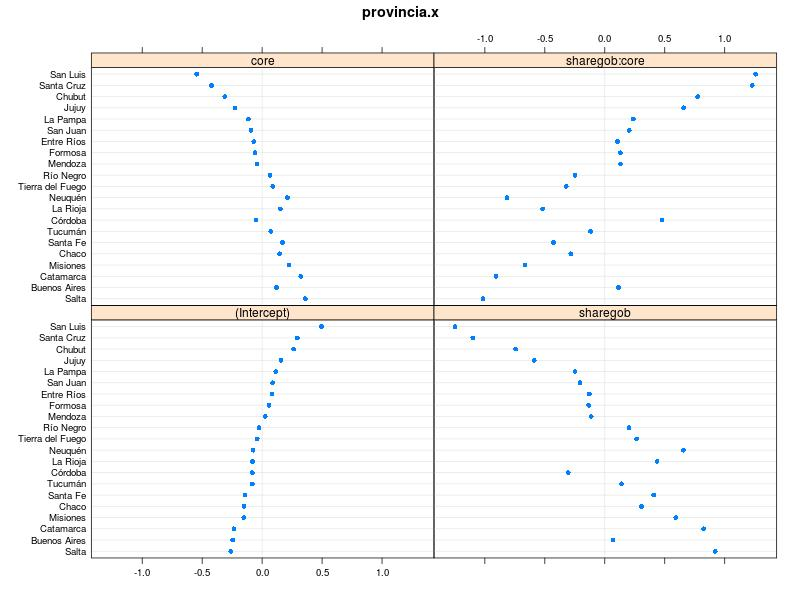
\includegraphics[scale=0.6]{effects1.jpg}
\end{figure}


\section{Methodological appendix}

One methodological issue was how to deal with different party lists
for the executive and legislative national elections. We ended up
having two measures. A strict measure where legislative vote for the
national ruling party (FPV) in each district was recorded if the same party/coalition
was competing at each legislative election. A broad
measure where legislative vote for the national ruling party (FPV) in
each district was recorded for the assigned to the party/coalition
which included Partido Justicialista. The first option is a better
choice for party coattails. The second option, however, allows us to
have full observations. We recorded the party/list that was recorded
for each instance where the FPV did not have its own legislative
list.





\bibliography{biblio}
\bibliographystyle{apalike}


\end{document}



% Table created by stargazer v.5.1 by Marek Hlavac, Harvard University. E-mail: hlavac at fas.harvard.edu
% Date and time: mié, jul 01, 2015 - 11:47:58 a.m.
% Requires LaTeX packages: dcolumn
\begin{table}[!htbp] \centering
  \caption{Gubernational Coattails}
  \label{}
\footnotesize
\begin{tabular}{@{\extracolsep{0}}lD{.}{.}{-2} D{.}{.}{-2} D{.}{.}{-2} D{.}{.}{-2} D{.}{.}{-2} D{.}{.}{-2} }
\\[-1.8ex]\hline
\hline \\[-1.8ex]
 & \multicolumn{6}{c}{\textit{Dependent variable:}} \\
\cline{2-7}
\\[-1.8ex] & \multicolumn{6}{c}{Presidential Vote Share} \\
\\[-1.8ex] & \multicolumn{1}{c}{\textit{OLS}} & \multicolumn{2}{c}{\textit{panel}} & \multicolumn{3}{c}{\textit{linear}} \\
 & \multicolumn{1}{c}{\textit{}} & \multicolumn{2}{c}{\textit{linear}} & \multicolumn{3}{c}{\textit{mixed-effects}} \\
\\[-1.8ex] & \multicolumn{1}{c}{(1)} & \multicolumn{1}{c}{(2)} & \multicolumn{1}{c}{(3)} & \multicolumn{1}{c}{(4)} & \multicolumn{1}{c}{(5)} & \multicolumn{1}{c}{(6)}\\
\hline \\[-1.8ex]
 sharegob & -1.19^{***} & -0.47^{***} & -1.16^{***} & -0.35^{***} & -0.26^{***} & -0.23^{***} \\
  & (0.06) & (0.08) & (0.06) & (0.05) & (0.08) & (0.09) \\
  & & & & & & \\
 core & -0.39^{***} & -0.09^{**} & -0.39^{***} & -0.05^{*} & 0.07^{**} & -0.04 \\
  & (0.03) & (0.04) & (0.03) & (0.03) & (0.03) & (0.03) \\
  & & & & & & \\
 encpprez & -0.18^{***} & -0.12^{***} & -0.18^{***} & -0.15^{***} & -0.14^{***} & -0.15^{***} \\
  & (0.004) & (0.01) & (0.004) & (0.004) & (0.005) & (0.004) \\
  & & & & & & \\
 PREZ\_FPV\_pre & 0.02 & -0.04^{***} & 0.08^{***} & -0.03^{**} & -0.01 & 0.02^{**} \\
  & (0.01) & (0.01) & (0.02) & (0.01) & (0.01) & (0.01) \\
  & & & & & & \\
 log(abs(dias\_prez\_gob + 1)) & -0.01^{***} & -0.02^{***} & -0.01^{***} & -0.01^{***} & -0.01^{***} & -0.01^{***} \\
  & (0.001) & (0.002) & (0.001) & (0.002) & (0.002) & (0.001) \\
  & & & & & & \\
 nbi & 0.85^{***} & 0.17 & 0.73^{**} &  &  &  \\
  & (0.29) & (0.38) & (0.29) &  &  &  \\
  & & & & & & \\
 sharegob:core & 1.21^{***} & 0.55^{***} & 1.18^{***} & 0.44^{***} & 0.30^{***} & 0.32^{***} \\
  & (0.06) & (0.08) & (0.06) & (0.06) & (0.06) & (0.11) \\
  & & & & & & \\
 Constant & 1.43^{***} &  &  & 1.03^{***} & 0.92^{***} & 0.97^{***} \\
  & (0.03) &  &  & (0.03) & (0.04) & (0.02) \\
  & & & & & & \\
\hline \\[-1.8ex]
Observations & \multicolumn{1}{c}{846} & \multicolumn{1}{c}{846} & \multicolumn{1}{c}{846} & \multicolumn{1}{c}{849} & \multicolumn{1}{c}{849} & \multicolumn{1}{c}{849} \\
R$^{2}$ & \multicolumn{1}{c}{0.84} & \multicolumn{1}{c}{0.59} & \multicolumn{1}{c}{0.85} &  &  &  \\
Adjusted R$^{2}$ & \multicolumn{1}{c}{0.84} & \multicolumn{1}{c}{0.28} & \multicolumn{1}{c}{0.84} &  &  &  \\
Akaike Inf. Crit. &  &  &  & \multicolumn{1}{c}{-2,445.63} & \multicolumn{1}{c}{-2,540.68} & \multicolumn{1}{c}{-2,757.83} \\
Bayesian Inf. Crit. &  &  &  & \multicolumn{1}{c}{-2,402.94} & \multicolumn{1}{c}{-2,488.50} & \multicolumn{1}{c}{-2,672.44} \\
Residual Std. Error & \multicolumn{1}{c}{0.07} &  &  &  &  &  \\
F Statistic & \multicolumn{1}{c}{645.77$^{***}$} & \multicolumn{1}{c}{81.62$^{***}$} & \multicolumn{1}{c}{652.23$^{***}$} &  &  &  \\
\hline
\hline \\[-1.8ex]
\textit{Note:}  & \multicolumn{6}{r}{$^{*}$p$<$0.1; $^{**}$p$<$0.05; $^{***}$p$<$0.01} \\
\end{tabular}
\end{table}




\begin{figure}
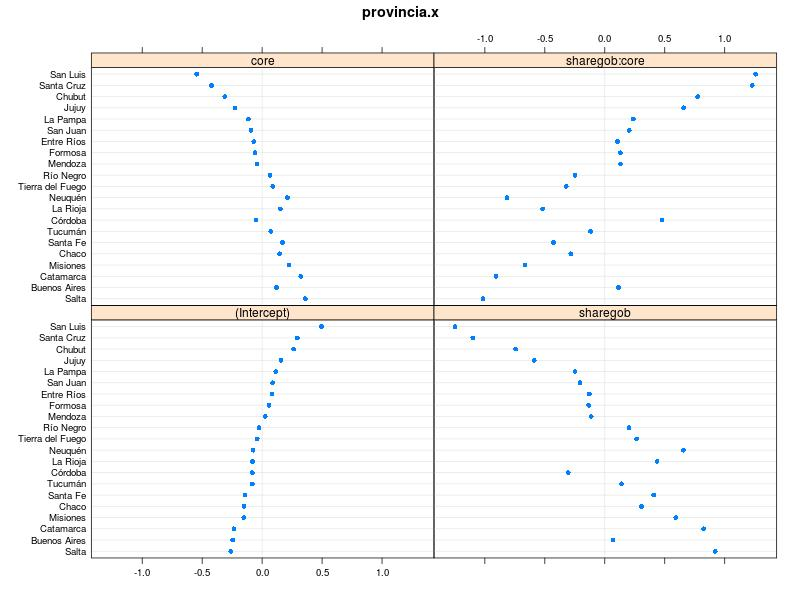
\includegraphics[scale=0.6]{effects1.jpg}
\end{figure}


Table \ref{tab:1} presents the results for the gubernatorial coattails. Model 1 runs the fully-pooled model assuming no structure in the data. Model 2-3 run the no pooling model using fixed-effects estimation for the parameters. Finally, models 4-5 run the mixed-effects models using linear mixed-effects estimation. Although we will focus our analyisis in the last two columns, the signs of the parameters are unchanged throughout all the models --there is some change in the size of the coefficients though. It is important to note the way our main variable of interest enters the model, as an interaction with the \textit{core} dummy for governor aligned with the national incumbent. Since we do not have data on the FPV candidate for governor, our \textit{sharegob} variable records the vote share of the incumbent governor in each department. The hypothesis we are interested in testing is whether the vote shares of governors aligned with the national incumbent have any effect on the latter vote shares. The way in which we model this is by including an interaction term between the \textit{sharegob} and \textit{core} variables. It can be seen that the direct effect of both variables is negative and significant although is interaction is positive and highly significant. In other words, the gubernatorial coattail effect --the vertical coattail- seems to be present for those cases where governors are aligned with the national incumbent. Other control variables have the expected sign. The effective number of competing parties in the Presidential election (\textit{encpprez}) is negative and significant meaning vote shares for Presidential election are smaller where vote is more atomized. The fraction of population with university education, a structural control available at the department-level, has a negative sign but is not significant. Finally, a variable controling for the concurrency between the President and gubernatorial election is measured as the distance (in days) between the two dates. It is significant and has a negative sign: more distant elections tend the vote share for President.

In Table \ref{tab:2}, we present the results for testing for congressional (lower house) coattail effects for the period 2003-2011. The baseline models include the same variables as in the gubernatorial coattail case except that we include the direct effect (without interaction) of the FPVs vote share for national deputies election. Aside from this difference, we run the same models as in Table \ref{tab:1}. The results are strikingly different from those in the previous table except for last column which is the expanded model estimated using mixed-effects. In fact, the main variable of interest, \textit{FPVDN} comes out with an odd negative sign and is almost never significant. However, the \textit{encp} is negative and highly significant, as was the case in the previous table. In the last column, it can be seen that the control variables all have the expected sign and are statistically significant. The FPV party vote share for national deputies variable is positive and significant: there seems to be a congressional coattail effect on the vote share of the national incumbent. This model fits the data significantly better the the baseline model given in column 4. Note that this results have been obtained by using only those districts where the party of that national incumbent (FPV) also explicitely ran congressional candidates\footnote{Despite this fact, there are districts where the national incumbent did not explicitely present a list or where the denomination of the competing party did not match the name of the incumbent party at the national level. To correct for this, we have run the same models in Table \ref{tab:2} but using a more inclusive measure which includes districts were either an explicit or implicit list could be considered as the party of the national incumbent.}

\section{Concluding remarks}


\end{document}
